% Standalone fragment; insert after verification_method.tex, before synthesis chapter.
% Sources are frozen final_rtl logs. Never substitute these charts for STA.
\clearpage
\section{最终冻结回归：21 项逐项图证}
本节对最终冻结快照的全部 21 项 testbench 补齐图证，来源为仓库 \code{docs/evidence/20260930/final_rtl/}。
程序核对成功状态、退出码、完成标记，以及全部日志和对应测试台的冻结 SHA。
每项列出计数、参考计算或断言对象及覆盖边界。\textbf{样本、输入码、断言、节拍和参数条件分别保留单位，不合成“总覆盖量”。}

\begin{figure}[H]\centering
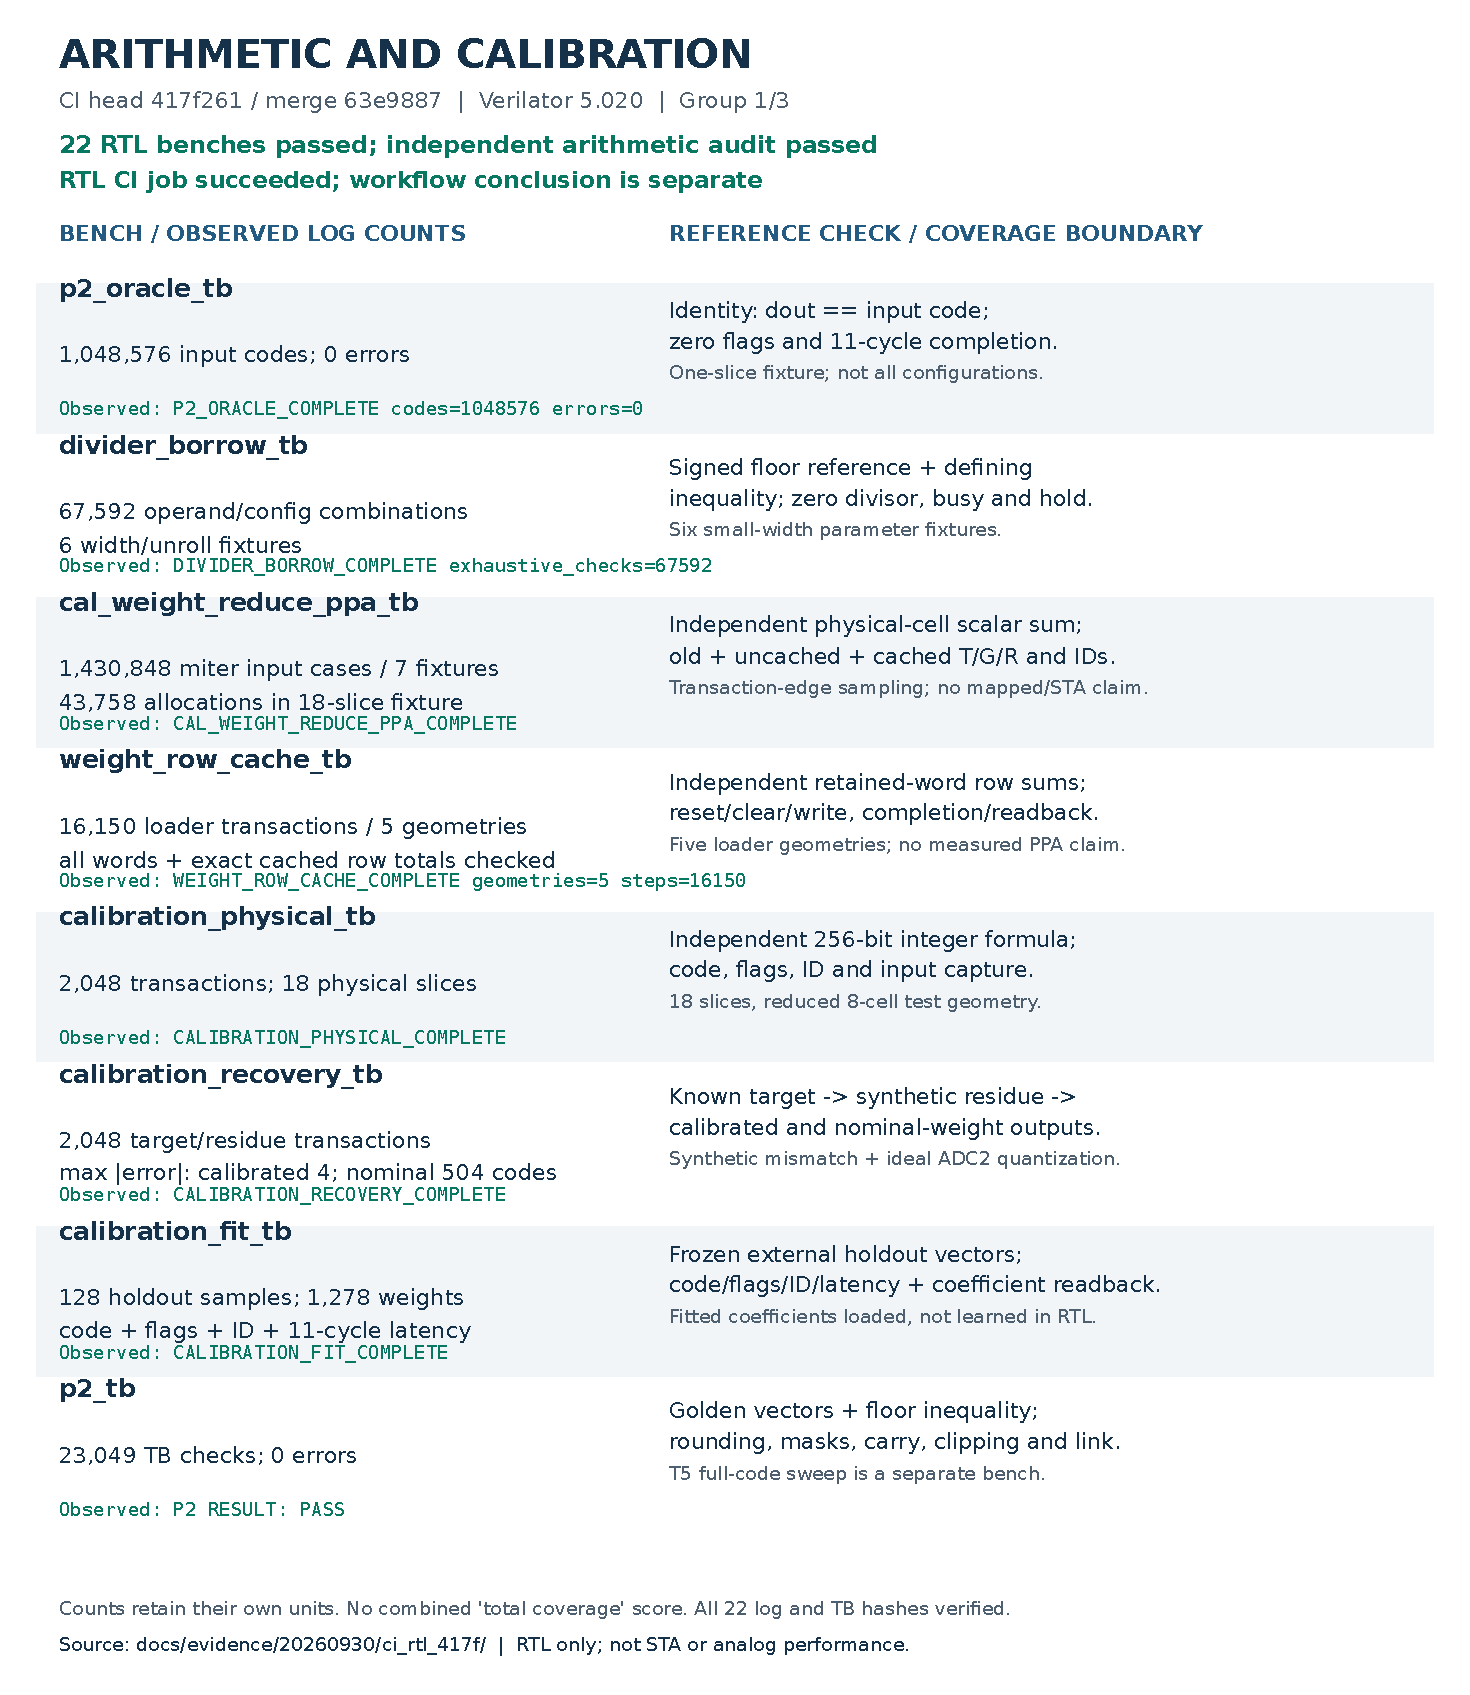
\includegraphics[width=.96\textwidth]{figures/final_regression_arithmetic.pdf}
\caption{算术与校准的七项最终回归。全码恒等测试只遍历一个简化配置；除法穷举覆盖六个小位宽参数实例；归约等价测试验证新旧结构逐位一致。物理权重、恢复和外部拟合测试分别使用独立宽整数公式、合成余差及冻结留出数据，不能相互替代。}
\label{fig:final-regression-arithmetic}
\end{figure}

\clearpage
\subsection{事务、取消与结构调度}
图\ref{fig:final-regression-protocol}中的 438 是结构顶层输出数，7,680 是该测试的检查节拍数，438 次延迟检查逐笔对应这些输出；三者不能相加为独立样本。
\code{review_recon_protocol_tb} 只打印完成标记，没有总检查计数，因此图中如实标为未记录。
\code{review_top_protocol_tb} 的 38 是测试台打印的固定输出数，图中不把它提升为独立的动态计数器证据。

\begin{figure}[H]\centering
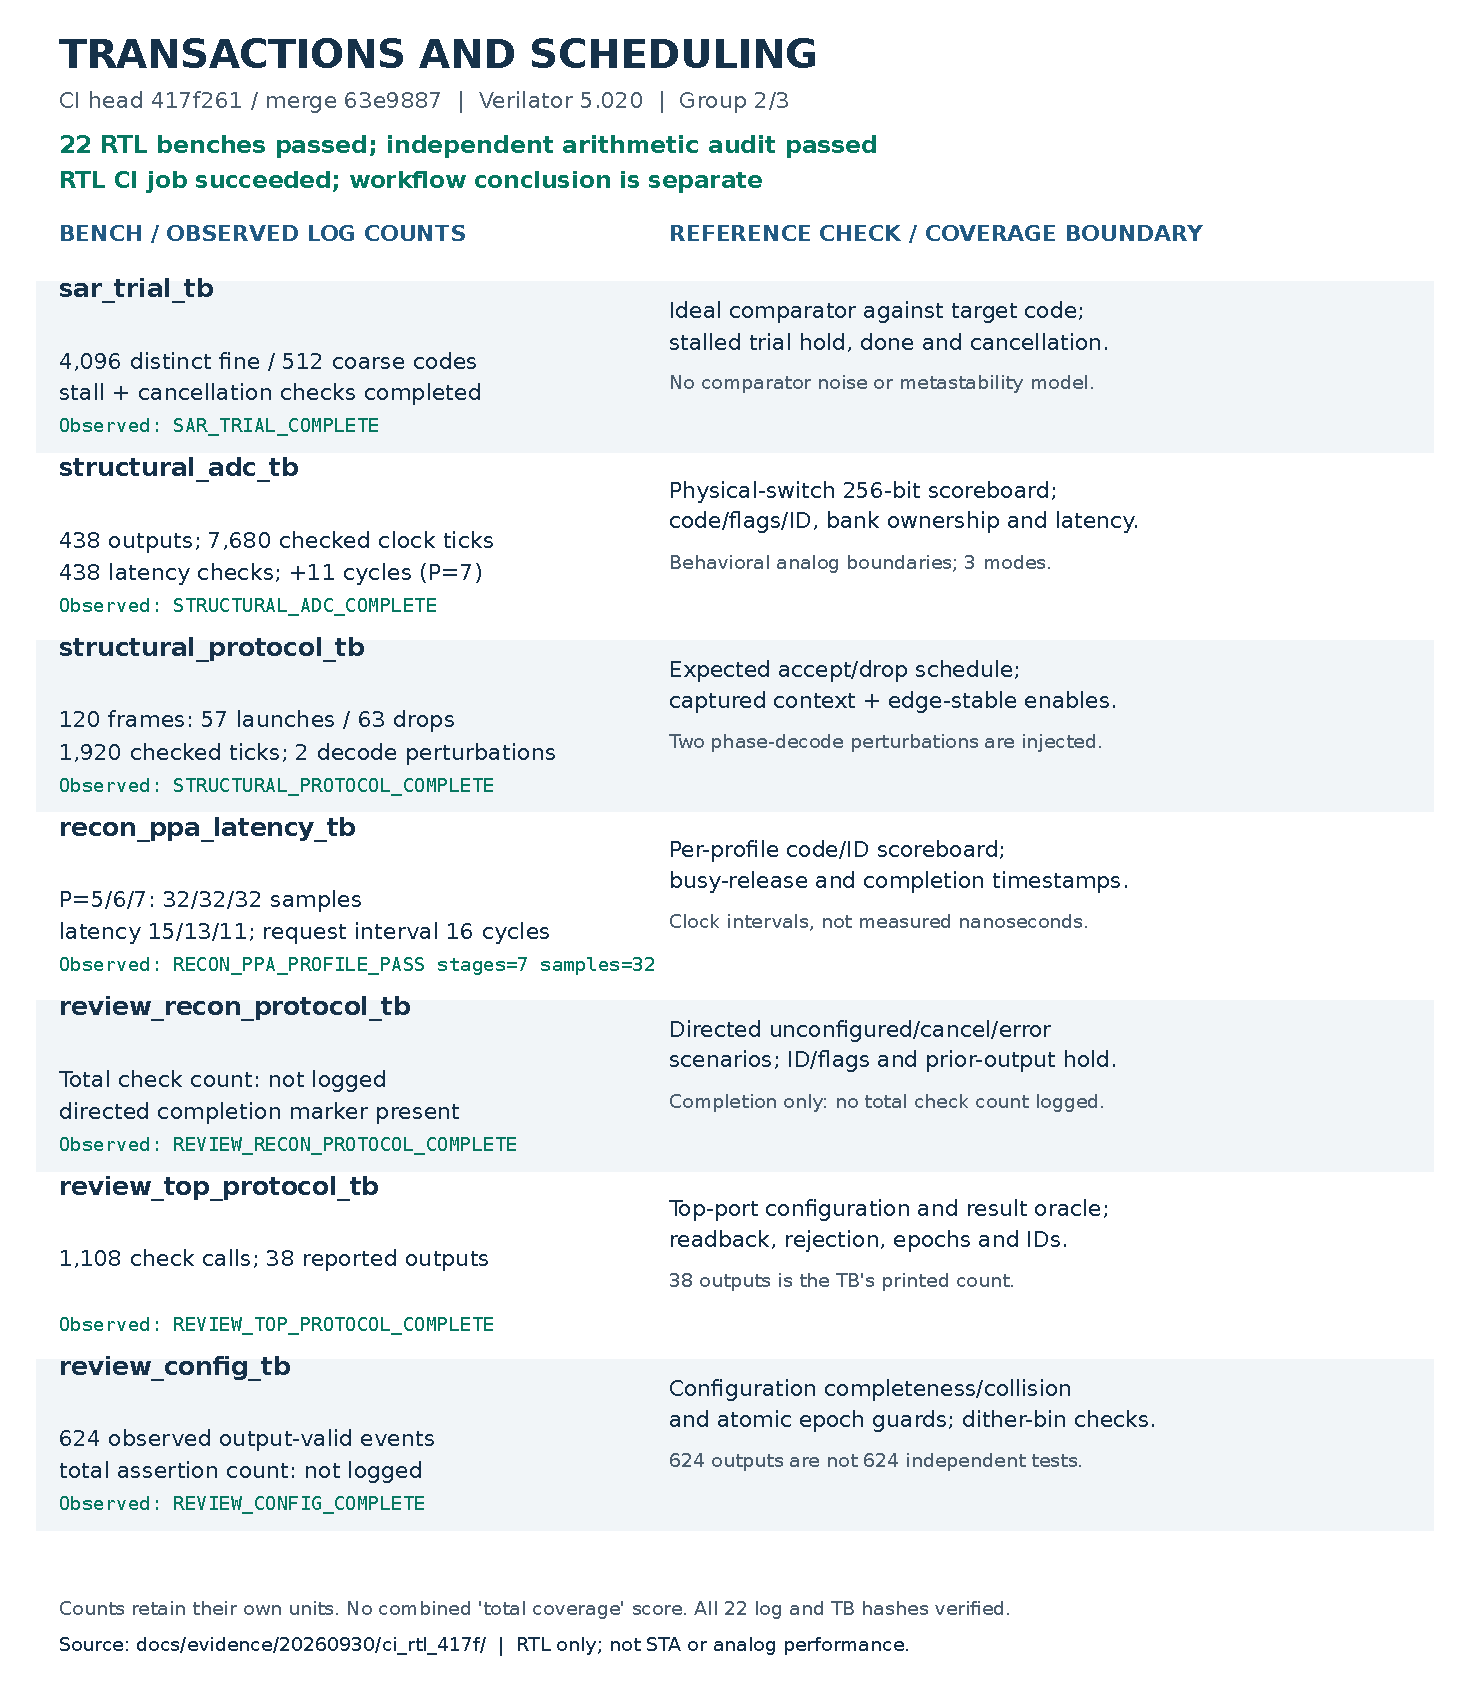
\includegraphics[width=\textwidth]{figures/final_regression_protocol.pdf}
\caption{事务和调度的七项证据。检查对象包括 SAR 停顿/取消、前后样本上下文隔离、ID/flags 对齐、无效配置屏蔽及 clear 后禁止旧 epoch 泄漏。展开级数 5/6/7 的输出延迟分别为 15/13/11 个完整时钟间隔，每项各 32 笔请求；这些是功能仿真的拍数，不是门级纳秒时延或 640\,MHz 签核。}
\label{fig:final-regression-protocol}
\end{figure}

\clearpage
\subsection{基础模块、配置和兼容顶层}
图\ref{fig:final-regression-system}保留所有旧测试的原始计数器含义。
例如外设测试依次打印的各小计是累计值，不能再次相加；dither 的七种幅度/种子条件分别在 200,000 个观测周期内接收 196,866 或 200,000 笔有效输出。
\code{tree_mapping_tb} 在此目录中是 Verilator RTL 回归；实际综合后单元检查须引用另存的 Vivado/XSim 证据。

\begin{figure}[H]\centering
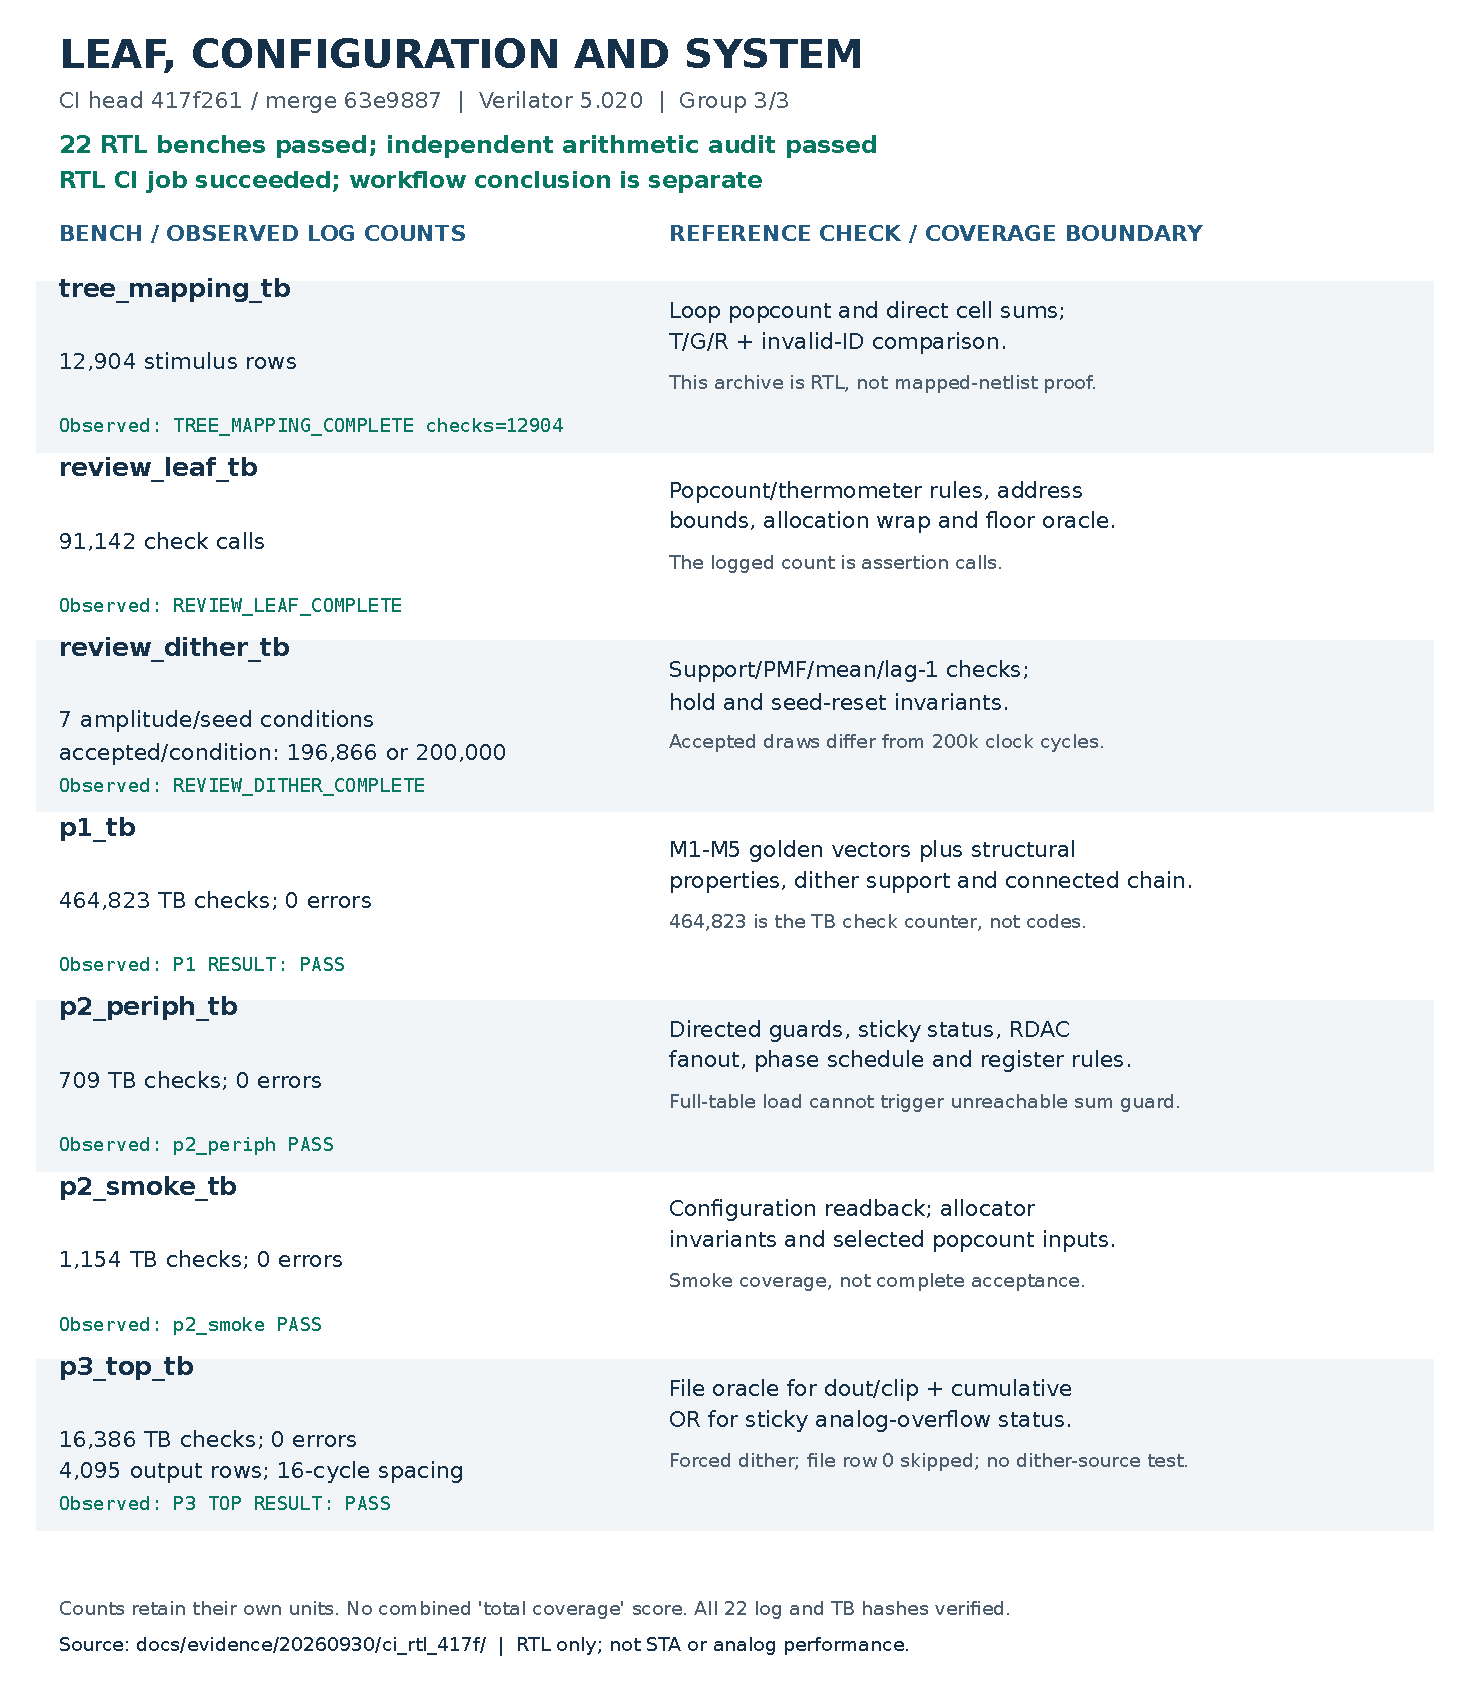
\includegraphics[width=\textwidth]{figures/final_regression_system.pdf}
\caption{基础模块、配置与兼容顶层的七项证据。兼容顶层比较 4,095 行输出，跳过向量文件第 0 行，并通过 force 注入 dither；因此不覆盖该模式下片内 dither 源。其 analog-overflow 按累积 OR 的粘滞口径比较，不能改用逐样本标志判断失配。}
\label{fig:final-regression-system}
\end{figure}

\clearpage
\subsection{日志中真正保留下来的定量观测}
图\ref{fig:final-regression-quantitative}只对存在的数据作图。
A、B 面板读取 \code{calibration_fit_tb.run.log} 的全部 128 条 \code{FIT_ROW}：逐样本实际码与期望码相同，flags 和 ID 无失配，延迟均为 11 拍；横轴是留出样本序号，不能称为模拟瞬态时间。
C 面板来自恢复测试的两个\emph{最大绝对误差}：标称权重为 504 码、校正权重为 4 码。日志没有逐样本误差分布，因此不能由两根柱子推导 RMS、SNDR 或 ENOB。

\begin{figure}[H]\centering
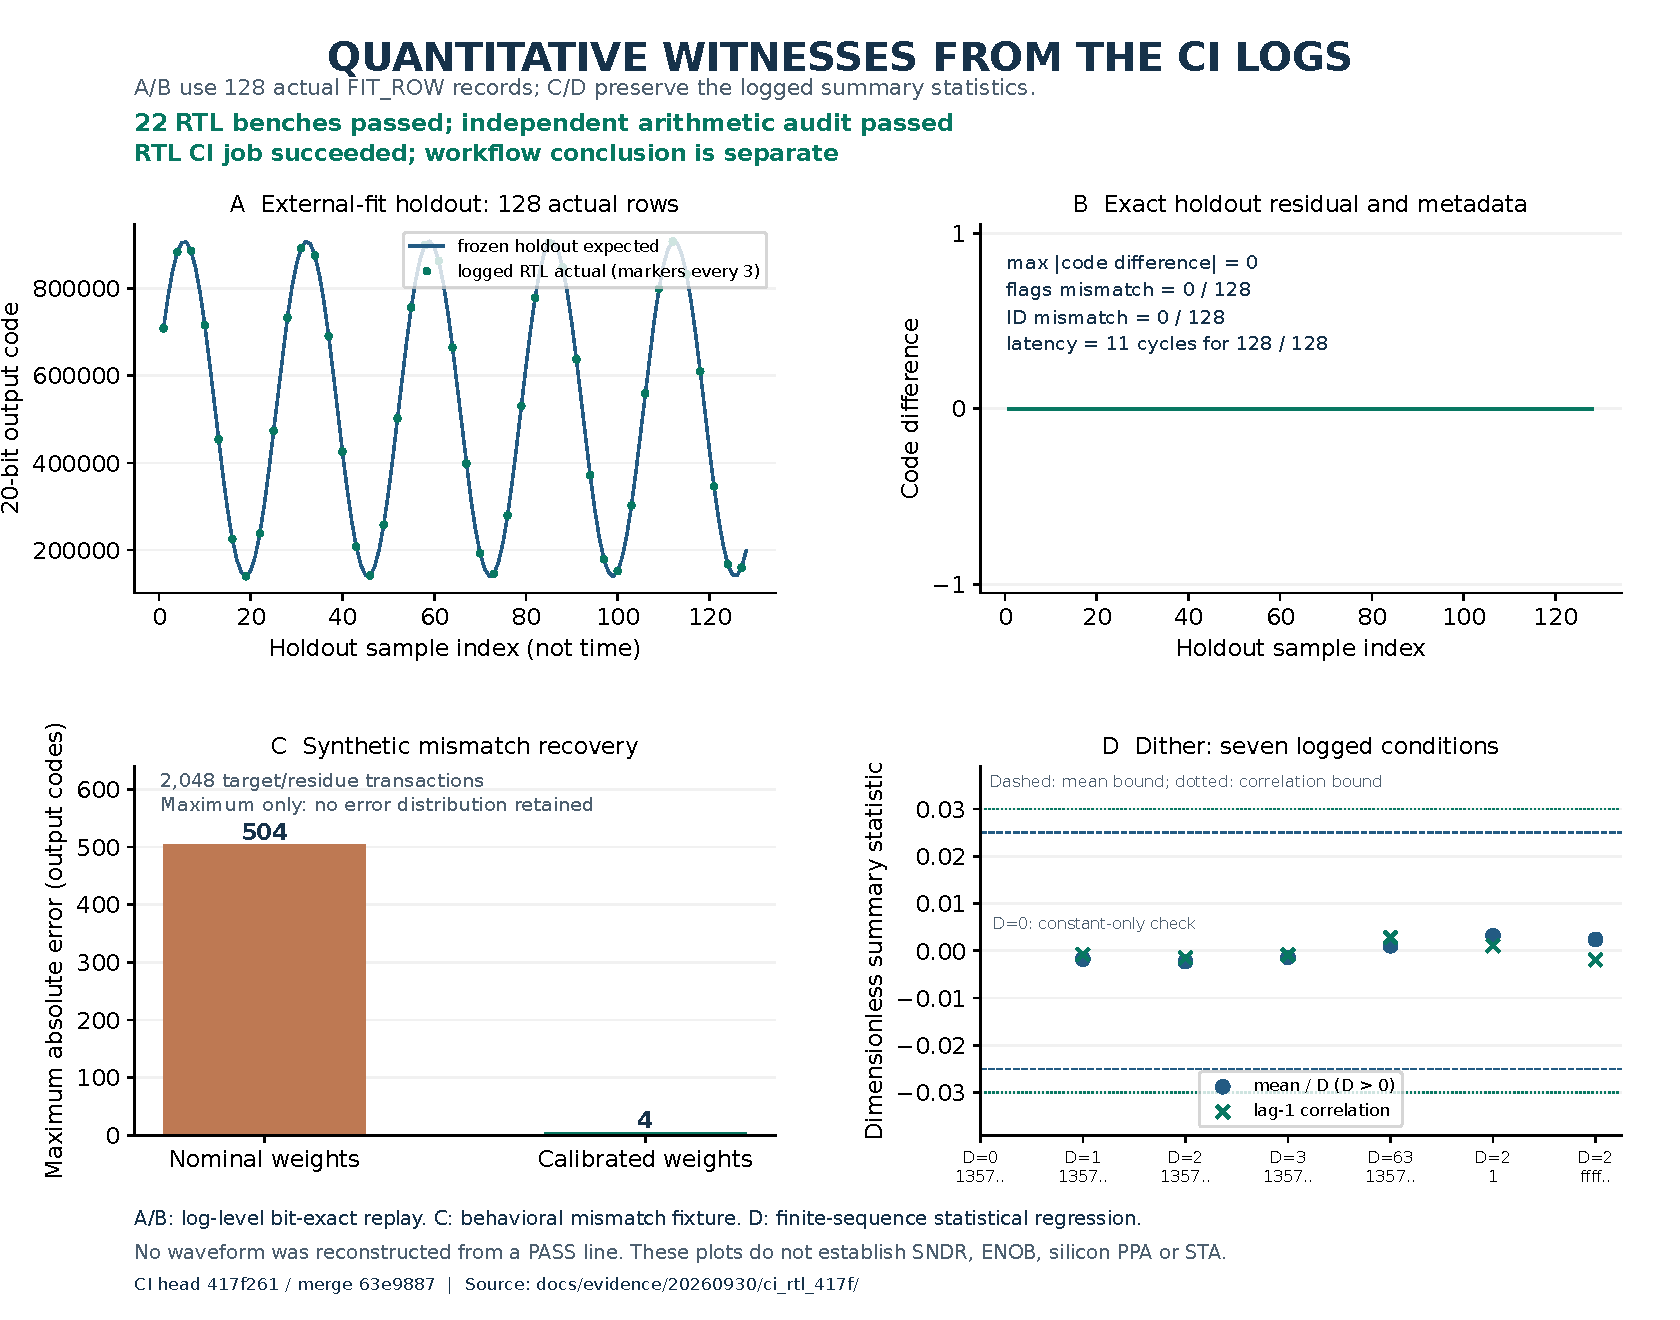
\includegraphics[width=\textwidth]{figures/final_regression_quantitative.pdf}
\caption{最终日志的定量观测。A/B 为逐样本序列；C 为 2,048 笔合成失配测试的最大误差摘要；D 为七种 dither 条件的已打印统计量，均值除以幅度 $D$，虚线与点线分别为测试台的 $\pm0.025$ 与 $\pm0.03$ 门限。$D=0$ 方差为零，测试台跳过相关性计算，图中亦不将打印的初始化零值画成有效相关系数。}
\label{fig:final-regression-quantitative}
\end{figure}

D 面板还保留两项限制：日志只给六位小数的均值/相关系数，图不声称更高精度；PMF 检查虽由测试台执行，但该日志未保留各直方图 bin，故不能从完成标记补画分布。其余三个矩阵没有时序序列，使用证据矩阵而非合成波形。

制图脚本为 \code{audit_figures/make_final_regression_evidence.py}，在报告目录运行即可重建四张 PNG/PDF；每张同名 \code{audit_figures/final_regression_*.sha256.json} 记录输入日志、测试台、结果清单、脚本和图件的 SHA-256，并保存解析后的计数和绘图数据。源码来源清单 SHA-256 为 \code{8c781172b9b9db072462da9305f98ec2580099da5d4577b206274ae533327caa}。
本节没有运行新的仿真，亦不提供 STA、模拟电路或硅片性能签核。
